
As was discussed in \sec\ref{sec:theory_www_production}, there are other decay
channels of the $WWW$ process besides the fully-leptonic decay channel,
which was the focus of Chapter \ref{sec:www}.  
In fact, one other decay channel for this process has been studied within 
ATLAS. This is the semi-leptonic channel where \wwwlljj. The details of this 
analysis are beyond the scope of this thesis. We can use the results of this channel,
however, along with those for the fully-leptonic decay channel, to obtain a stronger measurement
on the overall SM $WWW$ total cross-section measurement and limits on the aQGC signal reported than
those reported for just the fully-leptonic 
channel in \sec\ref{sec:measurement} and \sec\ref{sec:aqgc_limit}. 


In this chapter we will first summarize the results of the semi-leptonic study. 
This will be followed by a statistical combination of the fully-leptonic and semi-leptonic
results leading to an improved  
measurement on the SM $WWW$ total cross-section and limits on the 
aQGC signal.




\section{Search for \wwwlljj}

The signal plus background predictions, systematic uncertainties,
and observed event yields in data are taken directly from 
\cite{Butler:2030159} and \cite{Liu:2022894} 
for the fully-leptonic and 
semi-leptonic channels, respectively.  
The predictions, combined uncertainties, and observed events in data are summarized together for all six signal regions in table~\ref{tab:sys_summary}.  
Statistical uncertainties are shown as a symmetric uncertainty on the central value. Systematic uncertainties are shown as an asymmetric uncertainty and are shown after taking the quadrature sum of all individual uncertainties. 
In the analysis, each systematic uncertainty is treated as an individual nuisance parameter and are NOT added in quadrature.  The presentation here serves only as a demonstration of the overall size of the systematic uncertainties for each source in the individual signal regions.




\begin{landscape}
\begin{table}[h!]
\centering
%\begin{adjustwidth}{-1.5cm}{-1cm}
\small
\renewcommand{\tabcolsep}{1pt}
\def\arraystretch{1.3}
\begin{tabular}{c||rcl|rcl|rcl|rcl|rcl|rcl}
\hline
 & \multicolumn{9}{c|}{Fully-leptonic} & \multicolumn{9}{c}{Semi-leptonic} \\
 & \multicolumn{3}{c|}{0 SFOS} & \multicolumn{3}{|c|}{1 SFOS} & \multicolumn{3}{|c|}{2 SFOS} & \multicolumn{3}{|c|}{$ee$} & \multicolumn{3}{|c|}{$e\mu$} & \multicolumn{3}{|c}{$\mu\mu$}\\ 
\hline\hline
$WZ$ &  $0.5860 $&$\pm$&$ 0.0042~^{+0.0646}_{-0.0648}$ &  $11.89 $&$\pm$&$ 0.14~^{+1.30}_{-1.27}$ &  $9.05 $&$\pm$&$ 0.13~^{+0.97}_{-0.98}$ & 0.74 &$\pm$&  0.13 $^{+0.44}_{-0.44}$  & 2.77 &$\pm$&  0.27 $^{+0.66}_{-0.65}$  & 3.28 &$\pm$&  0.29 $^{+0.66}_{-0.71}$ \\[0.2cm] 
Other Prompt &  $0.214 $&$\pm$&$ 0.012~^{+0.020}_{-0.019}$ &  $0.780 $&$\pm$&$ 0.022~^{+0.110}_{-0.109}$ &  $0.602 $&$\pm$&$ 0.021~^{+0.099}_{-0.096}$ & 0.46 &$\pm$&  0.05 $^{+0.16}_{-0.15}$  & 1.33 &$\pm$&  0.1 $^{+0.37}_{-0.38}$  & 1.33 &$\pm$&  0.15 $^{+0.38}_{-0.32}$ \\[0.2cm] 
Charge Flip &  $0.0350 $&$\pm$&$ 0.0011~^{+0.0113}_{-0.0111}$ &  $0.0 $&$\pm$&$ 0.0~^{+0.0}_{-0.0}$ &  $0.0 $&$\pm$&$ 0.0~^{+0.0}_{-0.0}$ & 1.13 &$\pm$&  0.13 $^{+0.24}_{-0.24}$  & 0.74 &$\pm$&  0.08 $^{+0.16}_{-0.16}$  & 0.0 &$\pm$&  0.0 $^{+0.0}_{-0.0}$ \\[0.2cm] 
$V\gamma$ &  $0.0 $&$\pm$&$ 0.0~^{+0.0}_{-0.0}$ &  $0.20 $&$\pm$&$ 0.13~^{+0.29}_{-0.13}$ &  $0.110 $&$\pm$&$ 0.096~^{+0.163}_{-0.288}$ & 0.75 &$\pm$&  0.35 $^{+0.21}_{-0.18}$  & 2.48 &$\pm$&  0.68 $^{+0.73}_{-0.74}$  & 0.0 &$\pm$&  0.0 $^{+0.0}_{-0.0}$ \\[0.2cm] 
Fake &  $1.51 $&$\pm$&$ 0.26~^{+1.40}_{-1.29}$ &  $1.90 $&$\pm$&$ 0.34~^{+1.90}_{-1.77}$ &  $0.49 $&$\pm$&$ 0.16~^{+0.47}_{-0.46}$ & 0.96 &$\pm$&  0.15 $^{+0.39}_{-0.39}$  & 2.04 &$\pm$&  0.22 $^{+0.89}_{-0.89}$  & 0.43 &$\pm$&  0.06 $^{+0.25}_{-0.25}$ \\[0.2cm] 
Signal &  $1.344 $&$\pm$&$ 0.015~^{+0.068}_{-0.074}$ &  $1.394 $&$\pm$&$ 0.016~^{+0.068}_{-0.07}$ &  $0.614 $&$\pm$&$ 0.010~^{+0.029}_{-0.033}$ 
& 0.46 &$\pm$& 0.03 $^{+0.07}_{-0.07}$  & 1.35 &$\pm$& 0.05 $^{+0.19}_{-0.19}$  & 1.65 &$\pm$& 0.06 $^{+0.3}_{-0.3}$ \\[0.2cm] 
\hline
Total Background &  $2.35 $&$\pm$&$ 0.26~^{+1.40}_{-1.30}$ &  $14.77 $&$\pm$&$ 0.39~^{+2.34}_{-2.20}$ &  $10.25 $&$\pm$&$ 0.23~^{+1.13}_{-1.20}$ & 4.04 &$\pm$&  0.42 $^{+0.69}_{-0.68}$  & 9.36 &$\pm$&  0.77 $^{+1.39}_{-1.39}$  & 5.04 &$\pm$&  0.34 $^{+0.80}_{-0.82}$ \\[0.2cm] 
Total Predicted &  $3.69 $&$\pm$&$ 0.26~^{+1.40}_{-1.30}$ &  $16.16 $&$\pm$&$ 0.39~^{+2.31}_{-2.16}$ &  $10.86 $&$\pm$&$ 0.23~^{+1.10}_{-1.17}$ 
& 4.51 &$\pm$& 0.43 $^{+0.69}_{-0.69}$  & 10.72 &$\pm$& 0.77 $^{+1.4}_{-1.4}$  & 6.69 &$\pm$& 0.34 $^{+0.85}_{-0.87}$ \\ \hline 
\hline
Data &  \multicolumn{3}{c|}{$5$} &  \multicolumn{3}{|c|}{$13$} &  \multicolumn{3}{|c|}{$6$} & \multicolumn{3}{|c|}{0} & \multicolumn{3}{|c|}{15} & \multicolumn{3}{|c}{6}\\ 
\hline
\end{tabular}







%\end{adjustwidth}
\caption{A summary of the expected yields compared to data for all six signal regions.  
Statistical uncertainties are shown as a symmetric uncertainty on the central value. Systematic uncertainties are shown as an asymmetric uncertainty and are shown after taking the quadrature sum of all individual uncertainties. 
}
\label{tab:sys_summary}
\end{table}
\end{landscape}


Most object and event selection related systematic uncertainties are treated as $100~\%$ correlated 
between the signal regions derived for the semi-leptonic channel and those in the fully-leptonic channel.
However, there are some systematic uncertainties which have been derived independently between the 
two channels (e.g. fake background prediction uncertainties). We have chosen to treat these
uncertainties as completely uncorrelated. A summary of the systematic correlation scheme is 
presented in Table~\ref{tab:systematic_correlation_scheme}.

\begin{table}[h!]
\centering
\small
%\begin{tabular}{c||c||c}
\begin{tabular}{c||c}
\hline
Uncorrelated & Correlated \\
%\multicolumn{2}{c||}{Uncorrelated} & Correlated \\
%Fully-leptonic & Semi-leptonic & \\
\hline\hline
Background Normalizations&Electron Energy Resolution\\
Charge Mis-Identification&Electron Energy Scale \\
Fake Background estimation&Electron Efficiency Scale Factor\\
 &Jet Energy Resolution\\
 &Jet Energy Scale \\
 &Jet Vertex Fraction\\
 &Jet Flavor and Pileup\\
 &b-tag Jet Scale\\
 &b-tag Jet Scale Factor\\
 &Missing Et Soft Terms Resolution\\
 &Missing Et Soft Terms Scale\\
 &Muon Momentum Resolution \\
 &Muon Momentum Scale\\
 &Muon Efficiency Scale Factor\\
 &Muon and Electron Trigger Scale Factors\\
 &Pileup Reweighting \\
 &Luminosity \\
\hline
\end{tabular}

\caption{List of systematic categories split by whether they are treated as uncorrelated or correlated 
in the statistical combination of the two decay channels. There is no relationship between the entries on the same row.  }
\label{tab:systematic_correlation_scheme}
\end{table}




\subsection{Cross-sections}
\subsubsection{Fiducial Cross Section}
\label{sec:fiducial_xsec}


As described in \cite{Butler:2030159} and \cite{Liu:2022894},
fiducial regions are defined for each channel that are designed to 
be close to the reconstruction
level signal selection.
The fiducial selections are determined at truth level using 
Rivet \cite{Buckley:2010ar}.
%copied from semi-leptonic note since we are using the same code.
The fiducial cross-sections do not include the branching fraction 
to $W\rightarrow\tau\nu$ decay.
The final fiducial selection is presented
for each channel of the fully-leptonic channel in Table~\ref{tab:fiducial_selection_3l}
and for the semi-leptonic channel in Table~\ref{tab:fiducial_selection_2l2j}.


\begin{table}[ht!]
\centering
\begin{footnotesize}
\begin{tabular}{|c||c||c||c|}
\hline
&  0 SFOS  	& 1 SFOS		  & 2 SFOS  \\
\hline 
\hline 
All & \multicolumn{3}{c|}{All} \\
\hline 
Tau Veto & \multicolumn{3}{c|}{$N_{\tau} < 1$} \\
\hline 
Fiducial Leptons & \multicolumn{3}{c|}{Exactly 3 leptons with $p_{T} > 20~\mathrm{GeV}$ and $|\eta|<2.5$} \\
\hline 
Lepton Overlap Removal & \multicolumn{3}{c|}{$\Delta R(\ell \ell) > 0.1$}\\
\hline 
Same-Flavor Mass &	$m_{\textrm{SF}} > 20$~GeV	& \multicolumn{2}{c|}{} \\
\hline 
Z-Veto                &  \multirow{2}{*}{$|m_{ee}-m_Z| > 15$~GeV} & No $m_{\textrm{SFOS}}$ with  & \multirow{2}{*}{$|m_{\textrm{SFOS}}-m_Z| > 20$~GeV} \\
($m_Z = 91.1876$~GeV) & 					  & $m_{Z}-35 \textrm{GeV} < m_{\textrm{SFOS}}<m_{Z}+20$~GeV	&  \\
\hline 
Missing $E_{T}$		& 		& $E_{T}^{Miss} > 45$~GeV & $E_{T}^{Miss} > 55$~GeV \\
\hline 
Lepton-Missing $E_{T}$ Angle 	& 	\multicolumn{3}{c|}{$|\phi(3l)-\phi(E_{T}^{Miss})| > 2.5$} \\
\hline 
Inclusive Jet veto	& \multicolumn{3}{c|}{$N_{jet} \leq 1$ with fiducial jets of $p_{T} > 25~\mathrm{GeV}$ and $|\eta| < 4.5$ } \\
\hline 
\end{tabular}

\end{footnotesize}
\caption{Description of fiducial selection for each of the fully-leptonic channels.  }
\label{tab:fiducial_selection_3l}
\end{table}

\begin{table}[ht!]
\centering
\begin{footnotesize}

\begin{tabular}{|c||c|}
	\hline
      Cut Name & Details \\
      \hline
      \hline
      Tau Veto & Remove any events associated with Tau's \\
      \hline
      Lepton Selection & At least 2 leptons with $P_T> 15$ GeV  \\
      \hline
      Jet Selection & At least 2 jets with $P_T> 15$ GeV \\
      \hline
      Same-sign Leptons & Leptons must have the same electric charge \\
      \hline
      Final Lepton Selection & Exactly Two leptons with $P_T > 30$ GeV, $|\eta|<2.5$ \\
      \hline
      $\Delta R_{\ell \ell}$ & $\Delta R_{\ell \ell} > 0.1$ to remove any possible faulty lepton containers \\
      \hline
      $M_{\ell \ell}$ & $M_{\ell \ell} > 40$ GeV \\
      \hline
      Z Veto & $ | M_{ee} - M_Z | < 20$ GeV (only for the $ee$ channel) \\
      \hline
      Final Jet Selection & Leading(Sub) jet $P_T> 30~(20)$ GeV and $|\eta| < 2.5$ \\
      \hline
      $\Delta R_{\ell j}$ & min $\Delta R_{\ell j} > 0.3$ \\
      \hline
      MET & MET $ > 55$ GeV (Not applied for the $\mu\mu$ channel) \\
      \hline
      $b$-jet Veto & Remove any events that contain any $b$-tagged jets \\
      \hline
      $\Delta R_{jj}$ & $\Delta R_{j j} < 1.5$ to make sure that the two jets come from the $W$ boson decay \\ 
      \hline
      $W$ mass window cut & Two leading jets should have 65 GeV $<M_{jj}<105$ GeV  \\
      \hline
      jet-jet rapidity & $|\Delta y(jj)| < 1.5$ \\
      \hline

\end{tabular}


\end{footnotesize}
\caption{Description of fiducial selection for each of the semi-leptonic channels.  }
\label{tab:fiducial_selection_2l2j}
\end{table}


%need to add references to the madgraph samples in the sample section
The fiducial cross-sections are evaluated using 
%{\sc VBFNLO}~\cite{Arnold:2011wj}~\cite{Arnold:2012xn},
%at LO in QCD with an NLO
%k-factor applied and compared to cross-sections evaluated
%alternatively using 
{\sc MadGraph}~\cite{Alwall_madgraph} at NLO weighted to CT10 NLO.
A summary of the signal samples and cross-sections are
presented in Table~\ref{tab:signal_sample_summary}.
The derived fiducial cross-sections are shown in Table~\ref{tab:fiducial_cross_sections}.  


%need to add 2l2j vbfnlo samples. add jet kinematics?
%need to unify treatment of k-factors
%what is the actual uncertainty on the 3l vbfnlo samples?  right now
%my stat uncertainty has a better precision than the number provided
% is there some k-factor uncertainty?
\begin{table}[ht!]
\centering
\begin{footnotesize}
\begin{tabular}{|cc||c|c|}
\hline
\multicolumn{2}{|c||} {Sample} &  Cross-section [fb] \\
\hline
\hline
%\multirow{2}{*}{VBFNLO LO} & $W^{+}W^{+}W^{-}\rightarrow l\nu l\nu jj$ & & &  \\
%                        & $W^{-}W^{+}W^{-}\rightarrow l\nu l\nu jj $&  & & \\
%\hline
%\multirow{2}{*}{VBFNLO LO} & $W^{+}W^{+}W^{-}\rightarrow l\nu l\nu l\nu$ & $4.95 \pm 0.007$& $\pt > 5$~GeV & $|\eta<45|$ \\
%                        & $W^{-}W^{+}W^{-}\rightarrow l\nu l\nu l\nu $& $2.65\pm0.003$ & $\pt > 5$~GeV & $|\eta<45|$ \\
%\hline
\multirow{4}{*}{MadGraph NLO} & $W^{+}W^{-}W^{+}\rightarrow \textrm{Anything}$ &$59.47\pm0.11$ \\
                        & $W^{-}W^{+}W^{-} \rightarrow \textrm{Anything}$& $28.069\pm0.076$ \\
                        & $W^{+}H\rightarrow W^{+}W^{+}W^{-}(*)\rightarrow\textrm{Anything}$ & $99.106\pm0.019$ \\
                        & $W^{-}H\rightarrow W^{-}W^{+}W^{-}(*) \rightarrow \textrm{Anything}$& $54.804\pm0.010$ \\
\hline
\end{tabular}

\end{footnotesize}
\caption{Details of signal samples used to study signal fiducial cross-sections. The phase space
used for generation is restricted such that jets required
to have $\pt > 10$~GeV with no requirements on the pseudo-rapidity. There are no kinematic
restrictions for leptons.}
\label{tab:signal_sample_summary}
\end{table}


\begin{table}[ht!]
\centering
\begin{footnotesize}
\begin{tabular}{|cc||c|}
\hline
    & Channel & Fiducial Cross-section [ab] \\
\hline\hline
\multirow{3}{*}{Fully-leptonic}& 0 SFOS &  $123.6 \pm 4.7$        \\
&1 SFOS &  $136.9 \pm 4.7$           \\
&2 SFOS &  $48.8 \pm 2.9$          \\
\hline
\multirow{3}{*}{Semi-leptonic}& $ee$ &  $50.4 \pm 2.5$ \\
& $e\mu$ &  $125.2 \pm 3.8$ \\
& $\mu\mu$ &  $129.9 \pm 3.9$ \\
\hline
\end{tabular}

\end{footnotesize}
\caption{Fiducial cross-sections derived in each signal region. Production modes are summed together to get one fiducial cross-section per channel.  }
\label{tab:fiducial_cross_sections}
\end{table}


\subsubsection{Total Cross-section}
\label{sec:total_xsec}
The common total cross-section for $WWW\rightarrow Anything$ is derived using the sum of the cross-sections
for both resonant and non-resonant production and for both charge modes as determined from the {\sc MadGraph} samples
listed in Table~\ref{tab:signal_sample_summary}. The total cross-section is thus
determined to be:
\begin{equation}
\sigma^{\textrm{Total}}_{\textrm{Theory}}= 241.47\pm0.13 ~(\textrm{Stat.}) ~^{+10.33}_{-6.08} ~(\textrm{PDF}) ~\pm 6.3 ~(\textrm{Scale}) ~\textrm{fb} %uncertainty?
\end{equation}
Note that this cross-section also includes both the fully-hadronic decay mode and the decay mode with only one leptonic 
$W$-boson decay, neither of which are studied in this analysis. The branching fractions for all $WWW$ decay modes are summarized in
Fig.~\ref{fig:branching_fractions}. Together, the semi-leptonic and fully-leptonic decay modes studied in this combination
account for about 25\% of the $WWW$ branching fraction.

\begin{figure}
\centering
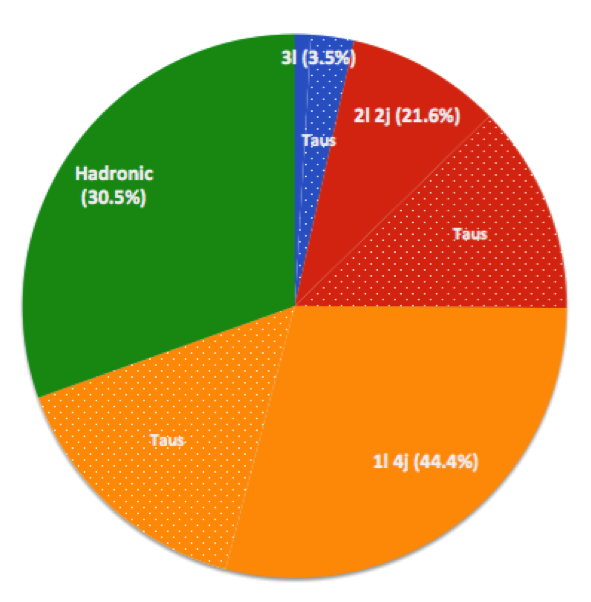
\includegraphics[scale=.8]{figures/combination/branching_fractions.png}
\caption{Pie chart showing the different decay modes contributing to the total cross-section for the $WWW$ process. The dotted areas indicate the portion of each decay mode which is due to the production of tau leptons.}
\label{fig:branching_fractions}
\end{figure}




\subsection{Correction Factor and Acceptance}
\label{sec:signal_efficiency_and_acceptance}

The correction factor, $C_i$, is defined for each channel, $i$,
as the ratio of the number of expected signal events measured
at the reconstruction level, $N_i^{\textrm{Reco}}$, listed
in Table~\ref{tab:sys_summary},
over the number expected from truth information, $N_i^{\textrm{Truth}}$:
\begin{equation}
\varepsilon_i = \frac{N_i^{\textrm{Reco}}}{N_i^{\textrm{Truth}}}
\end{equation}
We also choose to define the acceptance, $A_i$, for each channel, $i$,
as the ratio of the fiducial cross-section, $\sigma^{\textrm{Fiducial}}_i$,
over the total cross-section, $\sigma^{\textrm{Total}}$, 
described in section~\ref{sec:total_xsec}:
\begin{equation}
A_i = \frac{ \sigma^{\textrm{Fiducial}}_i }{ \sigma^{\textrm{Total}}}
\end{equation}
The overall acceptance is then simply sum of the acceptance in the individual channels
\begin{equation}
A = \sum_i A_i
\end{equation}

Using the reconstructed signal yields listed in Section~\ref{sec:inputs} and the fiducial
cross-sections generated using MadGraph
from Table~\ref{tab:fiducial_cross_sections}, we
arrive at the correction factors and acceptances listed in Table~\ref{tab:signal_efficiencies_and_acceptances}.
The overall acceptance is found to be $A = 2.547 \times 10^{-3} \pm 0.039 \times 10^{-3}$.


\begin{table}[ht!]
\centering
\begin{tabular}{|cc||c|c|}
\hline
%& Channel & Signal Efficiency, $\varepsilon_i$  & Acceptance ($\times 10^{-4}$), $A_i$\\
& Channel & $C_i$  & $A_i$ ($\times 10^{-3}$)\\
%&         & $\varepsilon_i$    &  $A_i$ \\
\hline\hline
\multirow{3}{*}{Fully-leptonic} & 0 SFOS &  $0.534 \pm .021$ & $0.512 \pm .019$ \\
				& 1 SFOS &  $0.500 \pm .018$ & $0.567 \pm .020$ \\
                                & 2 SFOS &  $0.615 \pm .038$ & $0.202 \pm .012$ \\
\hline
\multirow{3}{*}{Semi-leptonic} & $ee$     & $0.450 \pm .037$ & $0.209 \pm .011$\\
                               & $e\mu$   & $0.531 \pm .026$ & $0.519 \pm .016$\\
                               & $\mu\mu$ & $0.626 \pm .029$ & $0.538 \pm .016$\\
\hline
\end{tabular}

\caption{Correction factors and acceptances derived separately for each signal region. The sum of all of the acceptance
in each bin is used to compute the overall acceptance, $A$. Only statistical uncertainties are shown.}
\label{tab:signal_efficiencies_and_acceptances}
\end{table}


\section{Combined Cross-section Measurement}

%\newcommand*\Diff[1]{\mathop{}\!\mathrm{d}#1~}
%\newcommand{\boldtheta}{\boldsymbol{\theta}}
%\newcommand{\thetas}{\boldsymbol{\theta}_s}
%\newcommand{\thetab}{\boldsymbol{\theta}_b}
%\newcommand{\curlyl}{\mathcal{L}}

%\subsection{Introduction}
In this analysis we seek to measure the total cross-section, $\sigma^{\textrm{Total}}_{\textrm{Observed}}$, for the WWW production process.
The observed cross-section is parameterized by looking at the signal
strength, $\mu$, which is related to the expected cross-sections
from section~\ref{sec:xsec} by the relation:
\begin{equation}
\sigma^{\textrm{Total}}_{\textrm{Observed}} = \frac{\mu}{A} \sum_{i\in \textrm{Channels}} \sigma^{\textrm{Fiducial}}_i
\label{eq:sigmatot}
\end{equation}
where $A$ is the acceptance
measured as discussed in section~\ref{sec:signal_efficiency_and_acceptance}.
Assuming a counting experiment in each bin $i$, the expected event count is given by:
% assuming a simple Poisson counting experiment with expectation for a given bin/channel, $i$:
%should the acceptance really be here?
\begin{equation}
%N^{\mathrm{exp}}(\mu,\boldtheta) = N^{\mathrm{exp}}(\mu,\curlyl_0,\Delta_{\curlyl},\thetas,\thetab) = \mu \sum_i \curlyl(\curlyl_0,\Delta_{\curlyl}) \cdot \frac{\sigma^{\mathrm{Fiducial}}_i}{A_i} \cdot \varepsilon_i(\thetas) + \sum_{i}\sum_{\mathrm{bkg}} N_{i}^{\mathrm{bkg}}(\thetab)
N^{\mathrm{exp}}_i(\mu,\boldtheta) = N^{\mathrm{exp}}_i(\mu,\curlyl_0,\Delta_{\curlyl},\thetas,\thetab) = \mu \cdot \bigg( \curlyl(\curlyl_0,\Delta_{\curlyl}) \cdot \sigma^{\mathrm{Fiducial}}_i \cdot C_i(\thetas) \bigg) + \sum_{\mathrm{bkg}} N_{i}^{\mathrm{bkg}}(\thetab)
\label{eq:poisson_expectation}
\end{equation}
where $C_i$ is the correction factor
and $\sigma^{\mathrm{Fiducial}}_i$ is the fiducial cross-section in each 
bin discussed in section~\ref{sec:fiducial_xsec}. The 
individual background expectations in a given bin/channel, $i$, are expressed simply by the number of events
for a given background as $N^{\mathrm{bkg}}_i$. 
The correction factors and background expectations are assumed to follow probability distributions described by shape parameters determined from dedicated measurements of the background normalizations and systematic uncertainties.  
The set of correction factor shape parameters are referred to as $\thetas$ while the set of normalization and shape parameters on the background expectations are referred to as $\thetab$.
The integrated luminosity, $\curlyl$, is assumed to follow 
a Gaussian distribution with nominal integrated luminosity, $\curlyl_0$, and width, $\Delta_{\curlyl}$. 
Collectively, we refer to all of these parameters, except for $\mu$ as the set of nuisance parameters, $\boldtheta = (\curlyl_0,\Delta_{\curlyl}, \thetas, \thetab)$. 

The discovery significance is tested using frequentist statistics
to estimate the degree of compatibility with the background only hypothesis~\cite{Cowan:1277304}.
The measurement and uncertainty are evaluated 
by using the shape of the profile likelihood ratio~\cite{PDG:2014} 
which is a function of the data and the signal strength.

\subsection{Profile Likelihood Ratio}
\label{sec:profilelhoodratio}

The likelihood used is constructed as follows:
\begin{equation}
L(\mu,\boldtheta) = \mathrm{Gaus}(\curlyl;\curlyl_0,\Delta_{\curlyl})~\prod_{i\in\mathrm{Chan}} \mathrm{Pois}(N_i^{obs}|N_i^{exp}(\mu,\boldtheta))~\prod_{j\in\mathrm{Sys}} \mathrm{Gaus}(\theta_j;\theta_j^0,1)
\label{eq:poisson_likelihood}
\end{equation}
using the HistFactory tool developed within ATLAS \cite{Cranmer:1456844}. Note that the systematic uncertainties are given Gaussian constraints with $\pm1\sigma$ uncertainties.

The basic form of the 
test statistic used for comparing hypotheses is called the profile likelihood 
ratio, $\lambda(\mu)$ and is defined as:
\begin{equation}
-2 \ln \lambda(\mu) = -2 \ln \frac{L(\mu,\hat{\hat{\boldsymbol{\theta}}}(\mu))}{L(\hat{\mu},\hat{\boldsymbol{\theta}})}
\label{eq:profile_likelihood_ratio}
\end{equation}
Note that it no longer depends on the nuisance parameters, $\boldsymbol{\theta}$,
and instead depends only on $\mu$. 
The negative of twice the logarithm of the profile likelihood ratio is used because
the logarithm is monotonic and typically easier to work with.
The presence of the nuisance parameters is handled in the profiling 
step when constructing the profile likelihood ratio,  which results 
in a smearing of the profile likelihood ratio contour. 
During profiling, the systematic uncertainties are
interpolated using a piecewise linear function for shape uncertainties
and a piecewise exponential function for the normalization uncertainties
in order to maintain a normalization that is greater than zero.
The denominator is the 
unconditional maximum likelihood (ML)
evaluated at the ML estimators $\hat{\mu}$ and $\hat{\boldsymbol{\theta}}$.
This quantity is a unique constant when specified for a given likelihood
and set of nuisance parameters.
Meanwhile, the numerator is the conditional ML which depends on $\mu$ and
evaluated at 
the conditional ML estimator for the set of nuisance parameters, 
$\hat{\hat{\boldsymbol{\theta}}}$, which itself depends on $\mu$.
Clearly, the profile likelihood ratio runs from $0 < \lambda(\mu) < 1$
with values close to $0$ showing more agreement with the background only
hypothesis and values closer to $1$ showing more agreement
with the signal hypothesis, $\mu$. 
When taking the negative log likelihood, the range
is mapped to the entire positive axis and inverted. This means
that values close to $0$ are more background-like and larger values are more-signal
like.  

The minimum of the negative log of the profile likelihood 
is taken as the measurement of the signal strength, while
the uncertainty on the measurement is taken from the shape of the 
negative log profile likelihood assuming the behavior in the asymptotic
limit can be used.  The asymptotic behavior of the profile likelihood 
is used to evaluate the final confidence interval. 


\subsection{Testing for Discovery Significance}
The rejection of the background-only hypothesis ($\mu = 0$) is used to estimate the significance of a possible observation of the signal.
For the purposes of this test, the following test 
statistic is used:
\begin{equation}
q_{0} = 
\begin{cases}
\hfill -2 \ln \lambda(0),\hfill & \hat{\mu} \geq 0 \\
0,\hfill & \hat{\mu} < 0
\end{cases}
\label{eq:q0}
\end{equation}
The test statistic is set to $0$ when $\hat{\mu} < 0$ to enforce
the notion that an observation which is less than the background
expectation should not be treated as signal like. The $p$-value in this case
tells us the degree of incompatibility with the background only hypothesis
and is defined as:
\begin{equation}
p_0=\int^{\infty }_{q_{0,\textrm{obs}}} f(q_0|\mu=0) \Diff{q_0}
\label{eq:pvalue}
\end{equation}
where $q_{0,\textrm{obs}}$ is the observed value of $q_0$ and 
$f(q_0|\mu=0)$ is the probability density of the test statistic $q_0$ under
the background only hypothesis which is evaluated using toy MC. %explain?
By examining the $p$-value one can say what the probability is 
that the deviation away from the background only hypothesis is due
to chance. A small probability suggests that such a fluctuation is
unlikely. Frequently one refers to the significance:
\begin{equation}
Z = \Phi^{-1}(1-p_0)
\label{eq:significance}
\end{equation}
where $\Phi^{-1}$ is the inverse of the Gaussian cumulative distribution function.
In this way, one may refer to $Z\sigma$ significance of a measurement where usually
$3\sigma$ is considered to constitute 'evidence' while $5\sigma$ constitutes
discovery.

The distribution of $q_0$ is shown in Fig.~\ref{fig:stat_measurement_significance} for the combination.  
The observed null p-value 
is found to be 0.1657 ($0.971~\sigma$) with an expected of 0.152 ($1.026~\sigma$) for the combination.

%this is with reduced systematics. what is the effect of adding or removing more?
%plot should be redone with a bigger range
\begin{figure}[ht!]
\centering
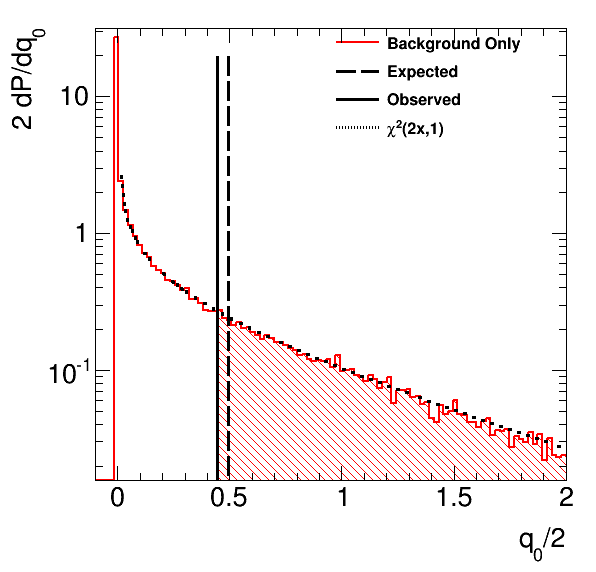
\includegraphics[width=0.70\columnwidth]{figures/combination/significance.png}
\caption{PDF of the background only hypothesis as a function of $q_0$ for the combination of all three channels. PDFs are determined 
using toy MC. The dashed black line represents the expected value of $q_0$ while the solid black line represents the observed value of $q_0$ seen in the data. The shaded area to the right
of this line represents the null p-value or the 
integral of the background hypothesis in the signal-like region.
The dotted black curve shows a $\chi^2$ distribution for 1 degree of freedom with which 
it can be seen is a good approximation of the 
the background only PDF.}
\label{fig:stat_measurement_significance}
\end{figure}

\clearpage

\subsection{Measurement and Uncertainty using Profile Likelihood Interval}
\label{sec:measurement}

The measured value of the signal strength is determined by looking at the minimum 
of the negative log profile likelihood 
for the combination of all channels. The size of the uncertainty on the 
measurement is taken by looking at the shape of the negative log 
profile likelihood contour which in general should follow a parabolic
shape centered about the minimum in the asymptotic limit. In this limit,
Wilk's theorem \cite{Wilk:1938}
can be used \cite{PDG:2014}
to determine that
the range of the 
uncertainty for a given number of Gaussian $\sigma$ can be related
directly 
to the negative profile log likelihood.  In particular, for 
a $1\sigma$ uncertainty, where $\% 68.3$ of experiments will fall, 
one expects that 
$|-\ln \lambda(\mu)| \leq 1/2$.
%\begin{equation}
%-2 \ln \lambda(\mu) = s^2
%\end{equation}
Note that even if the contour is not distributed symmetrically about the minimum
value, invariance of the likelihood under 
transformations like $g(\hat{\mu},\hat{\boldsymbol{\theta}})$ where $g$ is some function, 
means the same conclusion still holds.
The value of $\mu$ is not forced to be positive definite and is left unrestricted. 

The profile likelihood contour is evaluated once without systematic uncertainties included
as nuisance parameters in order to estimate the size of the measurement uncertainty purely 
from statistical effects and then a second time with the systematic uncertainties included
as nuisance parameters whose errors are constrained to be Gaussian and then 
profiled out. The contour with systematic uncertainties included represent
the total uncertainty and the systematic uncertainty is determined by assuming that
the total uncertainty is formed from the statistical and systematic uncertainties being added
in quadrature.
%The negative log likelihood contours as well as their uncertainties are shown for the individual channels in
%Fig.~\ref{fig:stat_measurement_interval_channels} 
The negative log likelihood contour is shown
for the combination of all six channels in 
Fig.~\ref{fig:stat_measurement_interval_combination}.
The expected value and uncertainties for the fiducial cross-section is:
\begin{equation}
\sigma^{\textrm{Total}}_{\textrm{Expected}} = 241.47 ~ ^{+232}_{-199} \stat ~^{+152}_{-153}\syst ~\textrm{fb}
\end{equation}
while the observed fiducial cross-section is:
\begin{equation}
\sigma^{\textrm{Total}}_{\textrm{Observed}} = 227.03 ~ ^{+202}_{-198} \stat ~^{+154}_{-160} \syst ~\textrm{fb}
\end{equation}

\begin{figure}[ht!]
\centering
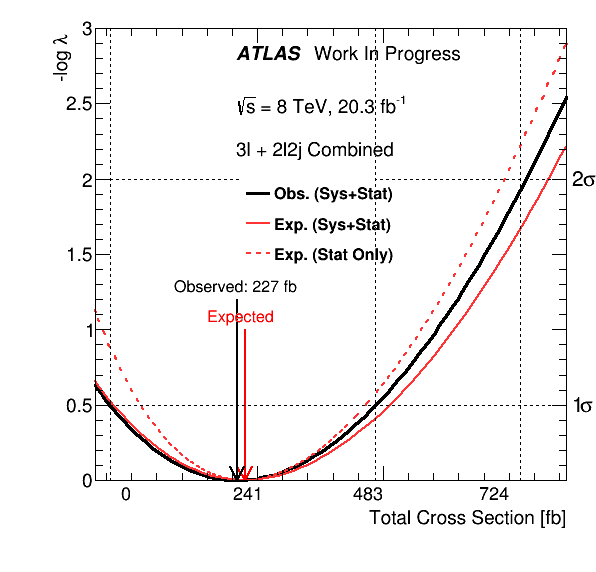
\includegraphics[scale=0.7]{figures/combination/interval_comb.png}
\caption{The profile likelihood contours evaluated as a function of the signal strength
for the combination of all three channels. 
The observed (black) and expected (red) contours are shown when considering only statistical uncertainty (dashed line) and when considering both statistical and systematic uncertainties (solid line).
The dotted black
lines pinpoint the location of the $1~\sigma$ and $2~\sigma$ total Gaussian uncertainties
on the measurement of the signal strength which corresponds to the minimum value of the contour.}
\label{fig:stat_measurement_interval_combination}
\end{figure}




\section{Combined aQGC Limits}

In addition to search for SM physics, the search for WWW signal allows us to put constraints on the beyond the SM physics using the effective Lagrangian approach. 

Using the following Lagrangian where ${\cal{O}}_i$ are dimension-six operators, ${\cal{O}}_j$ are dimension-eight operators,
\begin{equation}
{\cal{L}} = {\cal{L}}_{SM} + \sum\limits_{i} \frac{c_i}{\Lambda^2} {\cal{O}}_i + \sum\limits_{j} \frac{f_j}{\Lambda^4} {\cal{O}}_j + \cdots
\end{equation}
we set limits to $f_{S0}$ and $f_{S1}$ dimensionless coefficients defined in the following Lagrangian terms. The limits on these coefficents have been set before by the ssWW from CMS, but they haven't been measured in ATLAS yet. The 6 dimensional are parameters are assumed to be zero since they are well constrained by di-boson production. 

\begin{equation}
 {\cal{L}}_{S0} = \frac{f_{S0}}{\Lambda^4} [(D_\mu\Phi)^\dagger D_\nu \Phi] \times [(D^\mu\Phi)^\dagger D^\nu \Phi]
  \label{eq:EffLag2}
 \end{equation}

\begin{equation}
 {\cal{L}}_{S1} = \frac{f_{S1}}{\Lambda^4} [(D_\mu\Phi)^\dagger D^\mu \Phi] \times [(D_\nu\Phi)^\dagger D^\nu \Phi]
 \label{eq:EffLag1}
\end{equation}

The effective Lagrangian doesn't guarantee the unitarity of the theory, In order to prevent non-physical results, unitarization has to be applied. The details of the unitarization can be found in section \ref{sec:Unit}.


\subsection{Unitarization Scheme}
\label{sec:Unit}
The effective Lagrangian can keep it's unitarity below a certain energy scale. Beyond this point a form factor has to applied to ensure unitarity. However after discussing with the VBFNLO authors, it was concluded that no good solution is curently available to ensure at which value of $\Lambda_{ff}$ the unitarity would be restored. So it was decided to study the limits on the aQGC parameters for different values of $\Lambda_{ff}$ ($1000~\GeV$, $2000~\GeV$, and $3000~\GeV$). The limits are therefor provided for each of these values and for the un-unitarized case.

% The effective Lagrangian can keep it's unitarity below a certain energy scale, the figure \ref{fig:formfactor} taken from ~\cite{Wen:2014mha} shows the energy scale where the unitarity would be violated. Beyond this point a form factor has to applied to ensure unitarity. The form factor is determined by calculating on-shell vector boson scattering process cross section and computing the zeroth partial wave of the amplitude. As unitarity criterion the absolute value of the real part of the zeroth partial wave has to be below 0.5.

% \begin{figure}[h]
% \begin{center}
% 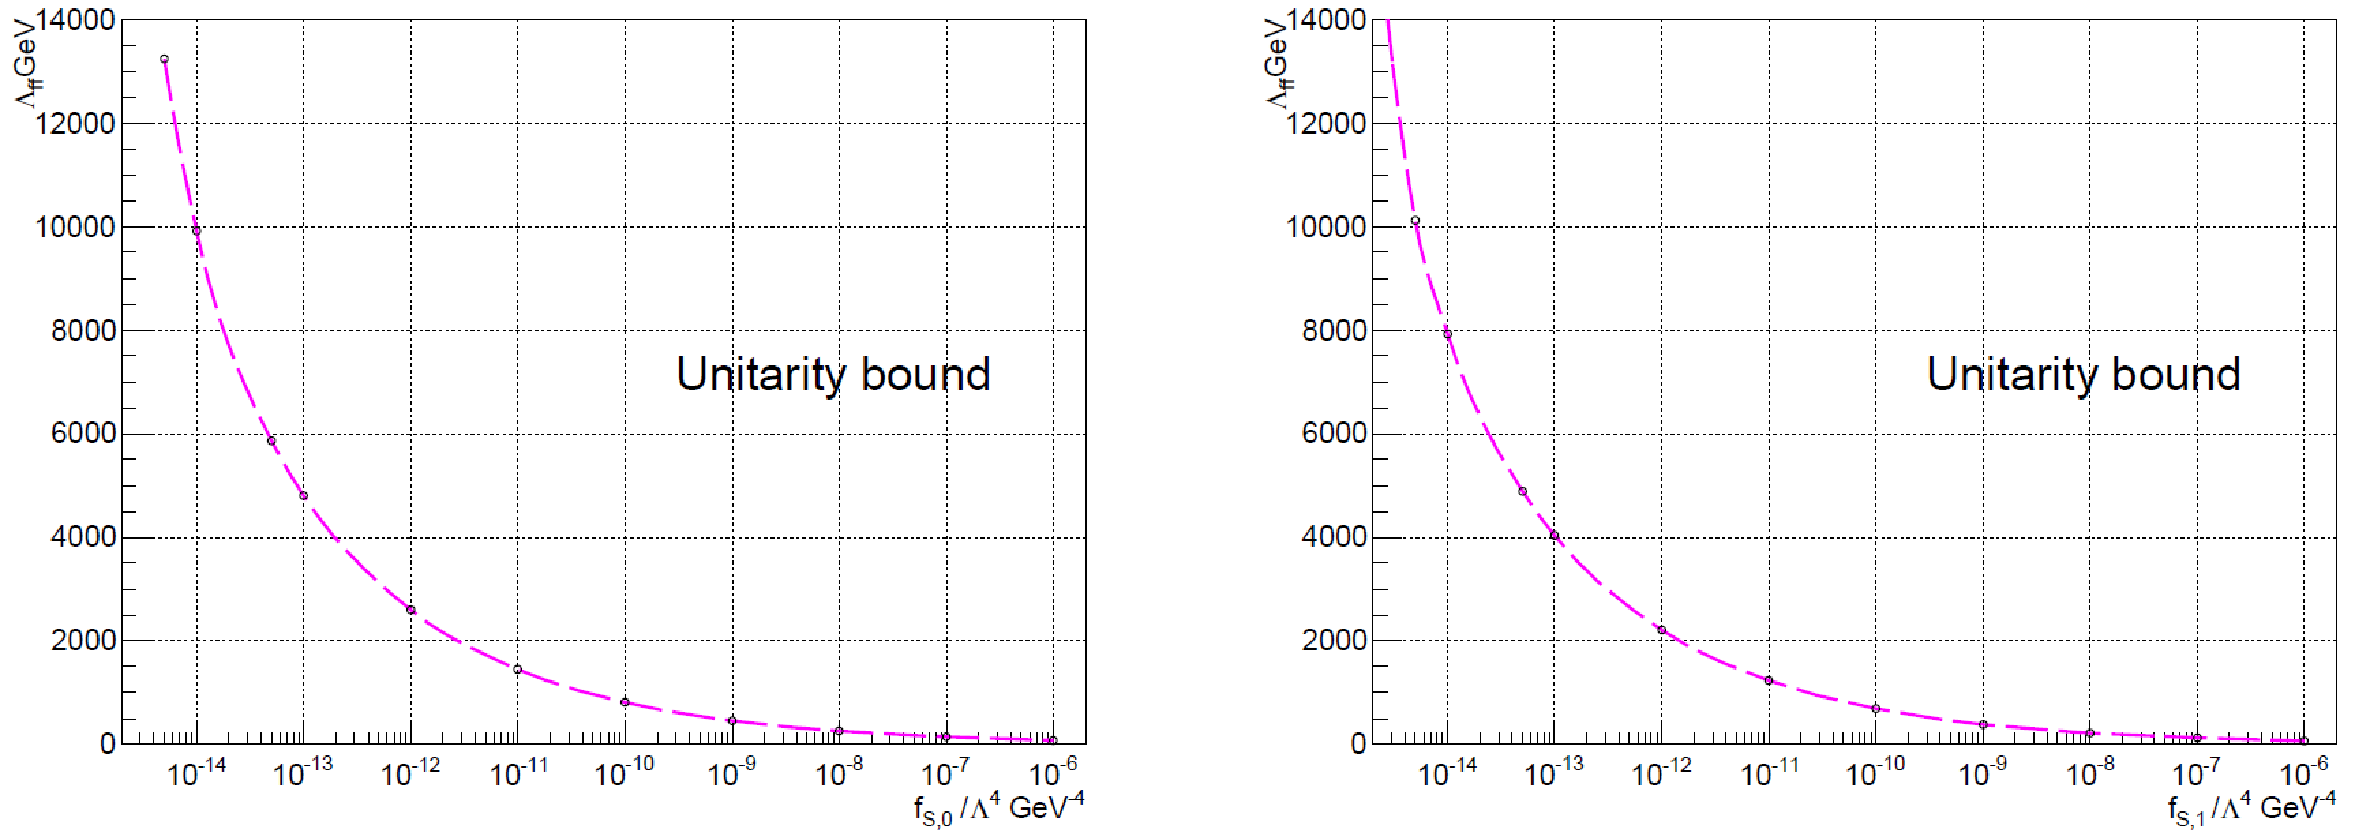
\includegraphics[width=0.9\textwidth]{figures/formfactor.pdf}
% \end{center}
% \caption{Unitarity bounds for ${\cal{L}}_{S0}$ and ${\cal{L}}_{S1}$.}
% \label{fig:formfactor}
% \end{figure}

\subsection{Measurement of aQGC}

The measurement of the aQGC limits are done using the TGClim tool. TGClim uses profile likelihood method to estimate the aQGC limits.It sets frequentist limits by using the profile likelihood method and conducting pseudo experiments to 
calculate a p-value (for the $95\%$ confidence level, the error on the p-value is $\pm0.2\%$). 
The likelihood function that is used to calculate these p-values is shown below:
\begin{equation}
 L(\mu,\theta) = \prod_{i=0}^m \text{Poisson}(N_{data}^i,\psi^i(\mu,\theta)) \times \left( \frac{1}{2\pi} \right)^m e^{-( \theta \cdot C^{-1} \cdot \theta)/2}
 \label{eq:likelihood}
\end{equation}
\begin{equation}
 \psi^i(\mu,\theta) = N^i_{sig}\times(1+\theta^i) + N^i_{bg} \times(1+\theta^{i+m})
\end{equation}
 where $\theta$ are nuisance parameters, and $C$ is 
the uncertainty matrix defined by $C_{ij} = \sum_k \sigma_{ik} \sigma_{jk}$.
The N$^i_{sig}$ is defined as a quadratic function of $f_{S0}$ and $f_{S1}$ variables given in the equation \ref{eq:Nsig} and these two parameters are our parameters of interest. 

\begin{equation}
  N_{sig} = w_0 + w_1f_{S0}^2+w_2f_{S1}^2+w_3f_{S0}+w_4f_{S1}+w_5f_{S0}f_{S1}
  \label{eq:Nsig}
\end{equation}

Here the $w_i$ are determined from a fit done to normalized and/or unitarized aQGC MC samples. 

The 95\% C.L. was determined for each anomalous coupling with the other coupling set to zero (1D limit) and simultaneously for both couplings at the same time (2D limit).

\subsubsection{Results}
The aQGC limits for different scales can be found  in table \ref{tab:aQGC-Lim} and figure \ref{fig:Ununit-aQGC}.

\begin{table}[h!]
  \begin{center}
  \tiny
    \begin{tabular}{  | l | c c | c c | c c c | c c c | }
      \hline
      Channel & \multicolumn{4}{c|}{Expected Limit} &\multicolumn{6}{c|}{Observed Limit} \\\hline 
      Units: $10^3\,$TeV$^{-4}$& \multicolumn{2}{c|}{Limits on F$_{s0}$} & \multicolumn{2}{c|}{Limits on F$_{s1}$} & \multicolumn{3}{c|}{Limits on F$_{s0}$} & \multicolumn{3}{c|}{Limits on F$_{s1}$}  \\\hline
      & Lower Limit & Upper Limit & Lower Limit & Upper Limit & Lower Limit & Upper Limit & Measured & Lower Limit & Upper Limit & Measured  \\\hline
      Scale 500  & -8.12 & 8.92 & -10.04 & 12.91 & -7.66 & 8.45 & 0.35  & -10.08 & 12.22 & 1.11 \\\hline
      Scale 1000 & -3.7 & 4.16 & -5.21 & 6.19 & -3.11 & 3.87 & 0.40 & -4.77 & 5.81 & 0.85  \\\hline
      Scale 2000 & -2.35 & 2.57 & -3.33 & 4.02 & -1.92 & 2.40 & 0.322  & -2.90 & 3.69 & 0.49 \\\hline
      Scale 3000 & -1.87 & 2.24 & -2.94 & 3.58 & -1.6 & 2.09 & 0.37 & -2.48 & 3.18 & 0.47  \\\hline
      Un-Unitarized & -1.59 & 1.91 & -2.54 & 3.09  & -1.27 & 1.76  & 0.34 & -2.10 & 2.71  & 0.40 \\\hline
    \end{tabular}
    \caption{Expected and observed limits on the aQGC Parameters.}
    \label{tab:aQGC-Lim}

  \end{center}
\end{table}

\begin{figure}[h!]
\begin{center}

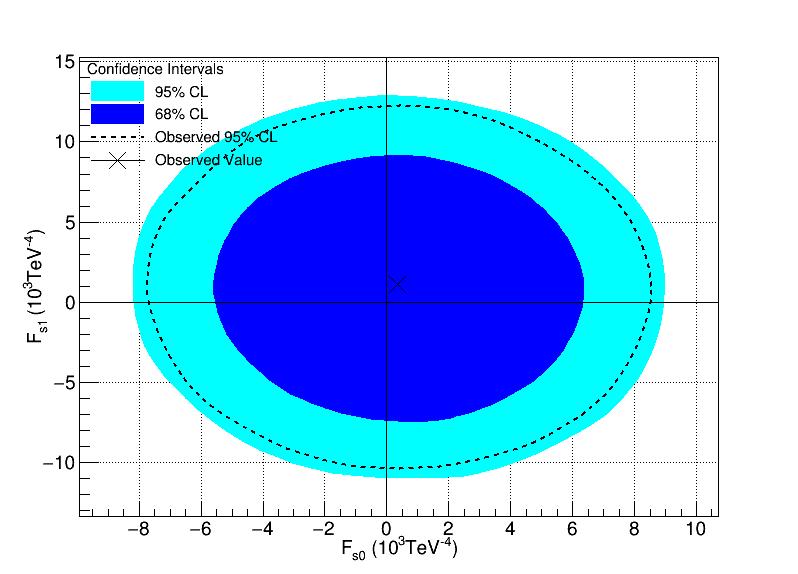
\includegraphics[width=0.45\textwidth]{figures/combination/Comb500-Lim.png}
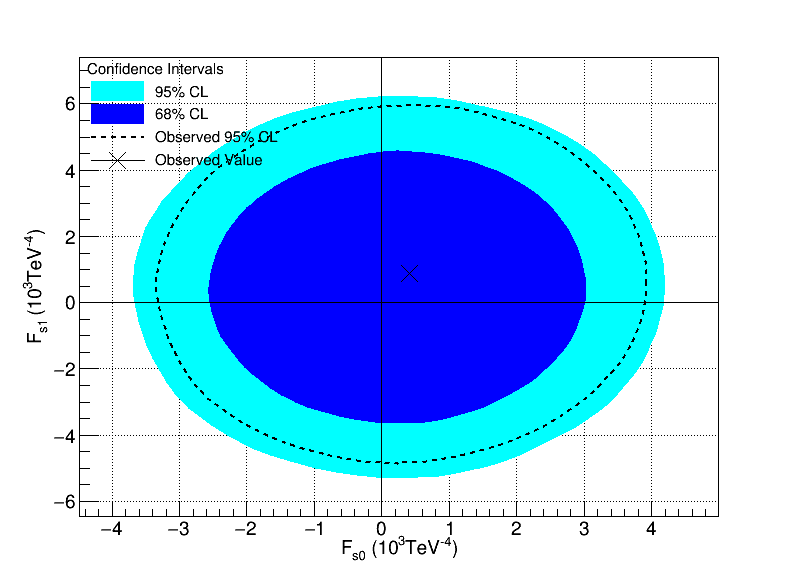
\includegraphics[width=0.45\textwidth]{figures/combination/Comb100-Lim.png}\\
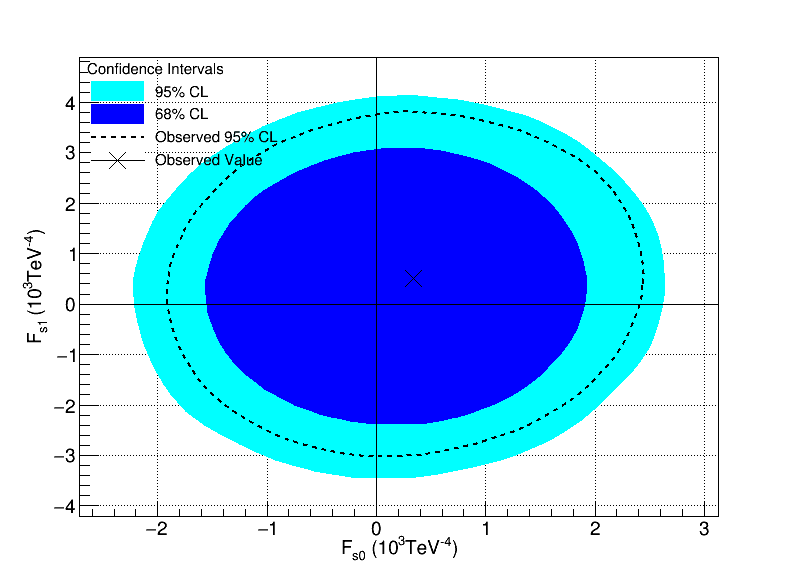
\includegraphics[width=0.45\textwidth]{figures/combination/Comb200-Lim.png}
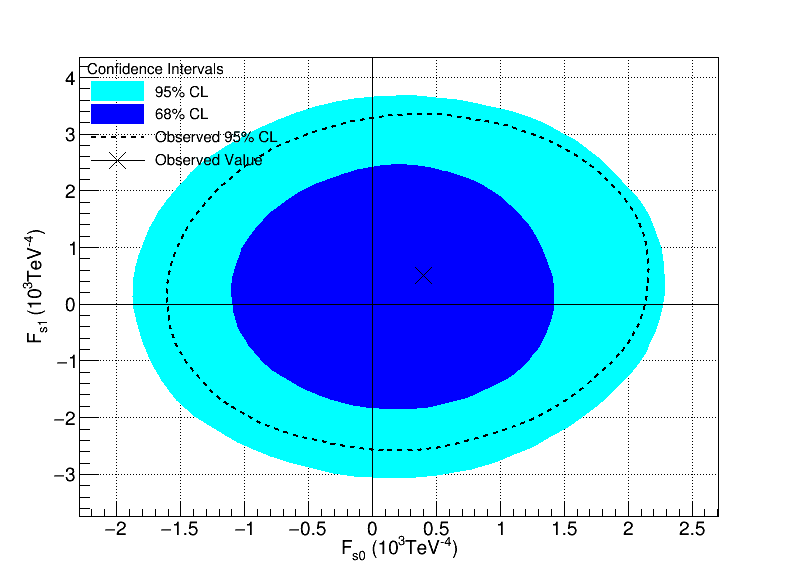
\includegraphics[width=0.45\textwidth]{figures/combination/Comb300-Lim.png}\\
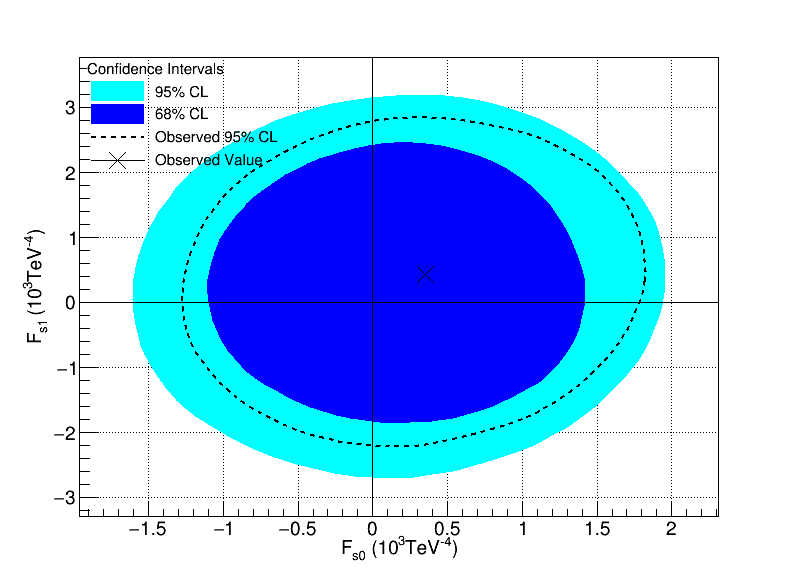
\includegraphics[width=0.45\textwidth]{figures/combination/CombUnit-Lim.png}
\end{center}
\caption{2D aQGC limits of Unitarized samples with scales 500,1000,2000,3000 and the Un-Unitarized Samples.(top left, top right, mid left, mid right, bottom)}
 \label{fig:Ununit-aQGC}
 \end{figure}



%%  LocalWords:  unitarization aQGC TGClim

